\documentclass[11pt,a4paper]{article}
\usepackage[T1]{fontenc}
\usepackage{lmodern}
\usepackage[margin=23mm]{geometry}
\usepackage{amsmath,amssymb}
\usepackage{xcolor}
\usepackage{tikz}
\usetikzlibrary{arrows.meta,positioning,calc}
\usepackage{hyperref}
\hypersetup{colorlinks=true,linkcolor=blue!45!black,urlcolor=blue!45!black}
\setlength{\parindent}{0pt}
\setlength{\parskip}{5pt plus 1pt}
\setlength{\emergencystretch}{2em}
\definecolor{water}{RGB}{205,231,241}
\definecolor{ink}{RGB}{30,62,79}
\tikzset{flow/.style={-{Latex},thick,ink}, equipment/.style={thick,ink},
         box/.style={draw=ink,rounded corners,align=center,inner sep=5pt}}
\title{Integrated process-control problems\\[4pt]{\large 45 problems with linked analytical and computational tasks}}
\author{Independent study collection}
\date{}
\begin{document}
\maketitle
\noindent Academic context: Intelligent Systems for Process Control and Automation, Prof. Michela Mulas. These newly written learning materials are not an official course plan and do not imply the professor's authorship, review or endorsement.

\tableofcontents\newpage
\clearpage\section{Unit 01: Modeling, identification and simulation}
\begin{center}
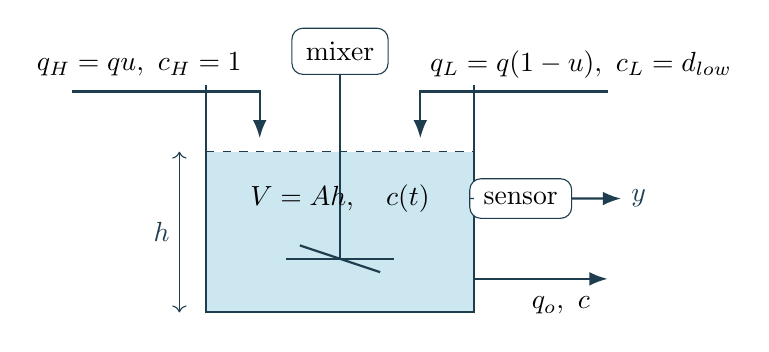
\begin{tikzpicture}[scale=0.85]
\fill[water] (0,0) rectangle (4,2.4);
\draw[equipment] (0,3.4)--(0,0)--(4,0)--(4,3.4);
\draw[ink,dashed] (0,2.4)--(4,2.4);
\draw[flow] (-2,3.3)--(0.8,3.3)--(0.8,2.6);
\draw[flow] (6,3.3)--(3.2,3.3)--(3.2,2.6);
\draw[flow] (4,0.5)--(6,0.5);
\draw[equipment] (2,3.8)--(2,0.8);
\draw[equipment] (1.2,0.8)--(2.8,0.8);
\draw[equipment] (1.4,1.0)--(2.6,0.6);
\node[box,fill=white] at (2,3.9) {mixer};
\node at (-1,3.7) {$q_H=qu,\ c_H=1$};
\node at (5.6,3.7) {$q_L=q(1-u),\ c_L=d_{low}$};
\node at (5.3,0.1) {$q_o,\ c$};
\node at (2,1.7) {$V=Ah,\quad c(t)$};
\draw[<->,ink] (-0.4,0)--node[left] {$h$}(-0.4,2.4);
\node[box,fill=white] (sensor) at (4.7,1.7) {sensor};
\draw[ink] (4,1.7)--(sensor);
\draw[flow] (sensor.east)--(6.2,1.7) node[right] {$y$};
\end{tikzpicture}
\end{center}
\noindent\textit{Physical boundary for the analytical tank. A constant-volume model requires inlet and outlet balance. Here the disturbance is low-feed concentration; the shared laboratory instead uses an additive disturbance to the complete inlet mixture. The sensor reading may have dynamics distinct from concentration.}

\subsection{Problem 01.1 - From vessel balances to an admissible simulation}
A tank initially contains 100 L at $c(0)=0.2$. The total inlet and outlet flows are 10 L/min and the high-concentration fraction becomes $u=0.7$. (a) Derive the concentration equation from total and solute balances, retaining the volume derivative until the end. (b) Obtain $c(t)$, its value at 10 min, and the time to reach 95\% of its total change. (c) Explain what changes if the outlet is fixed at 8 L/min; derive the new volume and concentration equations and identify which transfer-function assumption fails.

\subsection{Problem 01.2 - A sampled model that respects concentration bounds}
Use the same tank with a held input. (a) Derive the exact sampled model for an arbitrary $T_s$ and prove interval invariance. (b) Compare its pole with Euler at $T_s=1$, 15 and 25 min. (c) A numerical model produces a negative concentration after a valid inlet change. Decide which evidence would distinguish an integration artifact from a wrong balance or inconsistent initial condition.

\subsection{Problem 01.3 - Identify a process without leaking the answer}
Noiseless input-output samples are $(c_k,u_k,c_{k+1})=(0.2,0.8,0.26)$ and $(0.26,0.1,0.244)$. (a) Estimate $a,b$ and identify the time constant if these are exact one-minute samples. (b) Show why equilibrium-only observations do not uniquely determine both parameters. (c) Design independent training, validation and test trajectories for a noisy experiment and state which model choices may use each split.

\subsection{Problem 01.4 - Disturbance linearization and sensor dynamics}
Let the low-concentration feed carry an unknown normalized concentration $d$. Its balance is $10\dot c=u+(1-u)d-c$. A concentration sensor obeys $2\dot y=c-y$. (a) Linearize around $(u,d,c)=(0.4,0,0.4)$ and obtain both measured-output transfer functions. (b) Find the steady concentration after $d$ rises to 0.1 with fixed $u=0.4$. (c) Explain why fitting a single first-order model to $u\mapsto y$ can distort controller tuning.

\subsection{Problem 01.5 - Choose an identification claim that the evidence supports}
A model gives test errors $e=[0.1,-0.1,0.2,-0.2]$ on $y=[0,1,0,1]$. (a) Compute SSE, MSE, RMSE, maximum absolute error and $R^2$. (b) Give a case where a small one-step error would coexist with poor free simulation. (c) Propose two checks that would make a comparison against a model from Kroll and Schulte meaningful, and one conclusion these four samples cannot support.


\clearpage\section{Unit 02: Feedback, stability and IMC tuning}
\subsection{Problem 02.1 - An IMC reference design with a physical actuator}
The tank operates initially at $c=u=0.4$ and the reference changes to 0.6. (a) Derive PI gains for $\lambda=5$ min and the nominal reference response. (b) Compute the immediate actuator command using the equilibrium integral state. (c) Repeat for a reference of 1.2 and explain which part of the nominal calculation ceases to predict the real response.

\subsection{Problem 02.2 - A stable continuous design with an unstable software choice}
For $K_p=2$, $K_i=0.2$ per minute, use the exact held-input plant and the explicit integral update in the lesson. (a) Derive the closed-loop matrix. (b) Evaluate its eigenvalues for $T_s=1$ min. (c) Test $T_s=10$ min and explain why the continuous-time stability proof is insufficient.

\subsection{Problem 02.3 - Recover from windup}
At one sample $I=0.9$, $e=0.2$, $K_p=2$, $K_i=0.2$, $T_s=1$ min. (a) Calculate requested and applied commands. (b) Calculate the next integral state without anti-windup and with $K_{aw}=0.5$ per minute. (c) Explain why back-calculation should use actual actuator feedback when the valve differs from the software saturation.

\subsection{Problem 02.4 - Delay uncertainty and a robustness budget}
An identified model is $P(s)=e^{-2s}/(10s+1)$. (a) Apply the stated approximate IMC-PI rule for $\lambda=5$ min. (b) Compare gains to the delay-free design. (c) Propose a reproducible experiment with delay ranging from 1 to 4 min and explain which result would disqualify the fast tuning even if nominal IAE is smaller.

\subsection{Problem 02.5 - Choose metrics before choosing the winner}
Controller A has absolute errors $[0.2,0.1,0.05,0]$ and applied inputs $[0.8,0.3,0.7,0.5]$. Controller B has errors $[0.2,0.12,0.06,0.02]$ and inputs $[0.6,0.58,0.55,0.52]$. Assume one-minute equal-duration intervals and an initial input of 0.4. (a) Compute rectangle-rule IAE and total input variation. (b) Compare $J=\mathrm{IAE}+0.1\,\mathrm{TV}(u)$. (c) Explain what a fair report must disclose about this scalar score.


\clearpage\section{Unit 03: Multiloop, multivariable, feedforward and cascade control}
\begin{center}
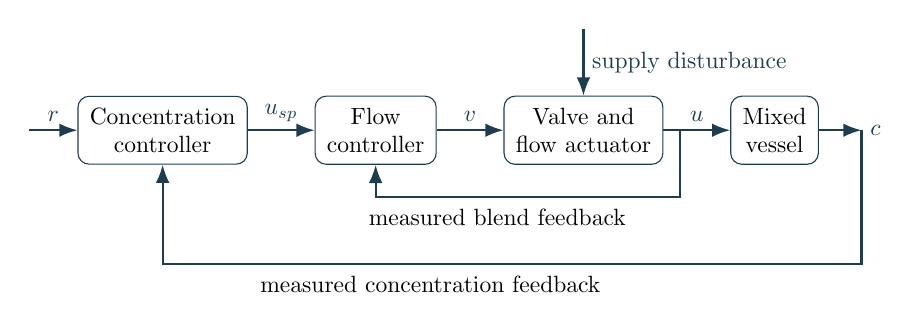
\begin{tikzpicture}[node distance=1.0cm,scale=0.85,transform shape]
\node[box] (outer) {Concentration\\controller};
\node[box,right=of outer] (inner) {Flow\\controller};
\node[box,right=of inner] (valve) {Valve and\\flow actuator};
\node[box,right=of valve] (tank) {Mixed\\vessel};
\draw[flow] (-2,0)--node[above] {$r$}(outer);
\draw[flow] (outer)--node[above] {$u_{sp}$}(inner);
\draw[flow] (inner)--node[above] {$v$}(valve);
\draw[flow] (valve)--node[above] {$u$}(tank);
\draw[flow] (tank)--++(1.3,0) coordinate (out) node[right] {$c$};
\draw[flow] ($(valve.east)+(0.25,0)$)--++(0,-1.0)-|(inner.south);
\draw[flow] (out)--++(0,-2)-|(outer.south);
\node at (5,-1.3) {measured blend feedback};
\node at (4,-2.3) {measured concentration feedback};
\draw[flow] ($(valve.north)+(0,1)$)--node[right] {supply disturbance}(valve.north);
\end{tikzpicture}
\end{center}
\noindent\textit{Cascade uses a measured inner variable. Both feedback paths are negative under the error conventions stated in the text.}

\subsection{Problem 03.1 - A feed composition disturbance}
The concentration target is 0.5. The low feed changes from $d=0$ to 0.2 while total flow remains constant. (a) Calculate the new blend fraction required for zero steady error. (b) Compare exact nonlinear feedforward with the linearization around $u=0.5,d=0$. (c) Determine what occurs if $d$ rises to 0.7 and the target is unchanged.

\subsection{Problem 03.2 - When perfect feedforward cannot be built}
Suppose $G_u=e^{-3s}/(10s+1)$ and $G_d=0.6e^{-s}/(10s+1)$. (a) Derive the ideal cancellation transfer function. (b) Explain the implementation obstacle. (c) Propose an implementable architecture and an experiment that separates feedforward benefit from ordinary feedback correction.

\subsection{Problem 03.3 - Design the inner flow loop before the outer loop}
A blend actuator has $\tau_v=2$ min and the vessel has $\tau=10$ min. Use $v=u_{sp}+K_f(u_{sp}-u)$. (a) Choose $K_f$ for an inner time constant of 0.5 min. (b) Derive the transfer functions from $u_{sp}$ and $w$ to $u$. (c) Discuss what a valve limit and sensor noise can invalidate in the desired bandwidth separation.

\subsection{Problem 03.4 - Pairing and decoupling a coupled process}
Use $K=\begin{bmatrix}1&0.6\\0.4&1\end{bmatrix}$. (a) Calculate its inverse and relative gain array. (b) Find the steady input change required for output change $[0.2,0]^T$. (c) If the available input deviations are each limited to $[-0.1,0.1]$, explain why independent output targets cannot be assumed achievable.

\subsection{Problem 03.5 - Select a structure with a fair information budget}
A concentration loop is affected by slow inlet-composition drift and rapid supply-pressure disturbances at its valve. Available upgrades are an upstream composition sensor and an inner flow sensor. (a) Map each sensor to the disturbance it can address. (b) Design a three-case comparison that attributes improvement to architecture rather than extra actuator range. (c) State why a static RGA from one operating point cannot settle the full design choice.


\clearpage\section{Unit 04: Constrained model predictive control}
\subsection{Problem 04.1 - Build the prediction matrices by hand}
For $c^+=ac+bu$, use $a=0.9,b=0.1$ and a prediction horizon of three. (a) Write $F$ and $G$ for $Y=[c_{k+1},c_{k+2},c_{k+3}]^T$. (b) Predict the sequence for $c_k=0.2$ and planned inputs $[0.5,0.7,0.4]^T$. (c) Explain which action a receding-horizon controller actually sends to the plant and when the other actions may change.

\subsection{Problem 04.2 - Solve a constrained one-step controller}
Use $a=0.9,b=0.1$, $c=0.2$, $r=0.8$, $u_{old}=0.4$ and $\rho=0.01$. (a) Derive and calculate the unconstrained optimum. (b) Enforce $0\leq u\leq1$ and $|u-u_{old}|\leq0.1$. (c) Compute the next concentration and explain why clipping the reference would solve a different problem.

\subsection{Problem 04.3 - Input increments and operating-point offsets}
A controller operates at $u=0.6$. (a) Write the difference matrix and initial-value vector for three planned absolute inputs. (b) Compare the penalties on $U=[0.6,0.6,0.6]^T$ when penalizing $U^TU$ and $(DU-d_0)^T(DU-d_0)$. (c) Explain the effect of using absolute inputs in a model identified in deviations.

\subsection{Problem 04.4 - A multivariable feasibility calculation}
At steady state $y=Ku$ with $K$ from Unit 03 and $0\leq u_i\leq1$. Target $y=[1.4,0.2]^T$. (a) Calculate the unconstrained input. (b) Prove that this target is infeasible. (c) Formulate a constrained steady target optimizer with output weights 4 and 1 and explain how it can support a dynamic MPC.

\subsection{Problem 04.5 - A solver failure is an operating event}
A constrained MPC normally finishes in 0.02 s but occasionally exceeds a 0.1 s sampling deadline. (a) Design a causal fallback and identify what state it must retain. (b) Explain how disturbance-state augmentation can address steady mismatch but not a missed deadline. (c) Specify a validation record that prevents an apparently good output plot from hiding solver failures.


\clearpage\section{Unit 05: Knowledge-based supervision and fuzzy control}
\subsection{Problem 05.1 - Diagnose a symptom without overclaiming a fault}
During a 20-minute experiment the concentration residual becomes positive, the commanded blend is 0.5, and measured blend remains 0.3. (a) Construct a rule that flags a flow-tracking problem after three consecutive samples. (b) Add a reset condition with hysteresis. (c) Explain which alternative hypotheses remain and what additional measurement would separate them.

\subsection{Problem 05.2 - A reproducible Sugeno control action}
Use the three memberships from the lesson with normalized error $e=0.3$. Single-input zero-order consequents are $z_N=-1,z_Z=0,z_P=1$. (a) Calculate every membership and the Sugeno output. (b) If this gives an input increment with $K_u=0.2$ and previous input 0.96, determine the requested and applied actions. (c) Explain why changing the error normalization changes the physical controller.

\subsection{Problem 05.3 - Mamdani centroid is not singleton averaging}
Two disjoint triangular output sets have centers -0.5 and 0.5, each base width 1 and height 1. Their supports are $[-1,0]$ and $[0,1]$. Minimum implication clips them at heights 0.8 and 0.2; aggregation is maximum. (a) Calculate each clipped area. (b) Calculate the centroid of the aggregate. (c) Compare with a Sugeno system using the centers as singleton consequents and the same firing strengths.

\subsection{Problem 05.4 - A fuzzy gain schedule with an explicit implementation}
Let $K_p(e)=1+2\min(|e|/0.2,1)$ and $K_i=K_p/10$. (a) Calculate the gains at errors 0, 0.1 and 0.3. (b) Write a sampled PI update with saturation and back-calculation using these gains. (c) State why testing the three fixed-gain linear models is useful but insufficient to validate the gain-scheduled loop.

\subsection{Problem 05.5 - Validate the rule surface before a closed-loop comparison}
A two-input fuzzy controller uses concentration error and its sampled difference. (a) Specify a grid-based test that checks correct sign, boundedness and coverage. (b) Explain why a symmetric rule table need not produce an odd control surface. (c) Design an ablation comparison between PI, fuzzy PI and fuzzy gain scheduling.


\clearpage\section{Unit 06: Neural modeling and control of dynamic systems}
\subsection{Problem 06.1 - A perceptron for a simple supervisory condition}
Inputs are binary indicators $x_1$ (high residual) and $x_2$ (flow mismatch); the desired alarm is their logical OR. (a) Give weights and bias implementing the desired truth table with output 1 when $w^Tx+b\geq0$. (b) Starting from $w=[0,0]$, $b=0$ and learning rate 1, calculate the update after the sample $x=[0,0],t=0$, then after $x=[1,0],t=1$. (c) Explain why this classifier does not localize a specific physical fault.

\subsection{Problem 06.2 - Differentiate a minimal neural predictor}
For one scalar regressor $x=0.5$, let $h=\tanh(w_1x)$, $\hat y=w_2h$, $w_1=1,w_2=0.8$, target $y=0.4$ and loss $L=(\hat y-y)^2/2$. (a) Compute the prediction. (b) Derive both weight gradients. (c) State how a finite-difference check and a separate validation trajectory catch different errors.

\subsection{Problem 06.3 - Fit and interpret a two-center RBF}
Use centers 0 and 1, width $\sigma=1$, no bias term, and training pairs $(x,y)=(0,0),(1,1)$. (a) Write the design matrix. (b) Solve for the two exact interpolation weights. (c) Explain what predictions far outside $[0,1]$ reveal about this architecture and why regularization changes interpolation.

\subsection{Problem 06.4 - A SOM organizes operating modes}
A two-unit SOM has prototypes $m_1=[0.2,0.3]^T$ and $m_2=[0.8,0.7]^T$. The normalized observation is $x=[0.3,0.4]^T$. Use learning rate 0.5, neighborhood weight 1 for the winner and 0.2 for the other unit. (a) Find the winner. (b) Calculate both updates. (c) Explain how training-data scaling and a subsequent fault label affect interpretation.

\subsection{Problem 06.5 - Put a neural prediction inside a bounded control decision}
A local learned model predicts $\hat c^+=0.9c+0.1u+0.02u^2$. At $c=0.4$, current $u=0.4$ and desired next concentration 0.5, use a Newton inverse step with $\gamma=1$. (a) Calculate the prediction, derivative and candidate input. (b) Enforce $0\leq u\leq1$ and $|u-u_{old}|\leq0.1$. (c) Give two reasons to retain a fallback even if this training model fits well.


\clearpage\section{Unit 07: Evolutionary optimization and controller tuning}
\subsection{Problem 07.1 - Binary resolution has a physical cost}
Encode $K_p\in[0,4]$ with four bits. (a) Decode chromosome 1001 and compute its resolution. (b) Find the nearest representable value to $K_p=2$. (c) Determine the minimum number of bits needed for resolution no greater than 0.02 and discuss the effect on search-space size.

\subsection{Problem 07.2 - Selection, crossover and mutation}
Two real chromosomes are $p_1=[2,0.2]$ and $p_2=[1,0.1]$. (a) Perform blend crossover with $\alpha=0.25$. (b) Apply mutation $[0.2,-0.15]$ and repair into bounds $K_p\in[0,4]$, $K_i\in[0.02,0.5]$ by projection. (c) Explain how a two-member tournament chooses among costs 0.6 and 0.4 and why recording the random seed is insufficient without the full evaluation protocol.

\subsection{Problem 07.3 - A fitness function that does not hide violations}
Candidate A has IAE 0.35, input variation 1.5 and no violations. Candidate B has IAE 0.30, variation 0.4 and one violation of a declared hard concentration limit. (a) Rank them under the soft cost $J=\mathrm{IAE}+0.1\,\mathrm{TV}$. (b) Rank them when the declared hard constraint is enforced. (c) Explain how to treat a simulation that becomes nonfinite rather than completing the horizon.

\subsection{Problem 07.4 - Tune MPC parameters without changing the ruler}
A chromosome contains horizon $N$, output weight $q$ and move weight $r_u$. Bounds are $N\in\{3,\ldots,20\}$, $q\in[0.1,10]$, $r_u\in[0.001,1]$. (a) Propose a valid decoding for real genes. (b) Explain why multiplying both weights by 10 does not change an exact unconstrained optimizer. (c) Define an external fitness that still permits meaningful comparison among these chromosomes.

\subsection{Problem 07.5 - Assess a stochastic tuning claim}
Two search methods each use population 20 for 15 evaluated generations, including their initial population. Method A reports only its best seed; B reports ten seeds. (a) Calculate the nominal evaluation budget per seed. (b) Propose a matched experiment and final test. (c) Explain why a lower best training cost does not prove superior generalization or a global optimum.


\clearpage\section{Unit 08: Integration, benchmark evidence and technical communication}
\subsection{Problem 08.1 - Design an integrated Blending Tank study}
Prepare a comparison of IMC-PI, feedforward PI, constrained MPC and one fuzzy or neural method on the hypothetical tank. (a) Define a common reference/disturbance protocol with a training period and a separate final test. (b) State the measurements each controller receives and how to disclose additional information. (c) Specify six reported outcomes and the minimum evidence required to reproduce them.

\subsection{Problem 08.2 - A biased model can have perfect VAF}
Measured targets are $y=[0,1,2,3]$ and a model predicts $\hat y=y+0.5$. (a) Compute RMSE, VAF and $R^2$ using population variances and the standard definitions. (b) Explain why the metrics disagree. (c) Propose an additional validation check and explain what to report for a constant-output test record.

\subsection{Problem 08.3 - Distinguish reproduction from a teaching model}
Consider three submissions: A implements the article's specified artificial recurrence with matching input/initial conditions; B simulates a wind rotor with an invented constant torque coefficient; C runs an official Tennessee Eastman implementation with a documented disturbance schedule. (a) Classify what each can support. (b) List metadata needed before comparing A or C with published scores. (c) Explain how B can still be useful without overstating its identity.

\subsection{Problem 08.4 - Cross-language agreement has several levels}
Python and Octave simulations differ by $10^{-7}$ in concentration but by 0.02 in a threshold-based settling time. MATLAB/Simulink has not yet run. (a) Explain a plausible cause of the settling difference. (b) Propose numerical and behavioral cross-language checks. (c) Write an accurate validation statement.

\subsection{Problem 08.5 - Make a defensible recommendation from mixed results}
In a fixed synthetic test family, a tuned controller reduces median IAE by 12\% but increases input variation by 40\%, misses two deadlines in 1,000 samples, and was tested at only one residence time. (a) State a supported conclusion. (b) Identify which additional experiments address generalization, timing and actuator wear. (c) Give a report outline that makes both the benefit and limitations inspectable.


\clearpage\section{Unit 09: Markov chains and hidden-state diagnosis}
\subsection{Problem 09.1 - Predict sensor regimes and interpret a stationary distribution}
A simplified sensor has states normal and drift, sampled every 0.2 min, with $P=\left[\begin{smallmatrix}0.9&0.1\\0.2&0.8\end{smallmatrix}\right]$ and $p_0=[1,0]$. (a) Explain the Markov and time-homogeneity assumptions, and calculate $P^2$ and the probability of drift after two steps. (b) Derive the stationary distribution and an expression for $p_n$; calculate $p_5$. (c) Find the expected consecutive duration of a normal episode. (d) Explain why stationarity does not mean that the sensor stops changing state, and give a two-state example with a stationary distribution but no convergence from $p_0$.

\subsection{Problem 09.2 - Separate expected lifetime from near-term fault probability}
For a different maintenance model, use states normal, degraded and failed, with $P=\left[\begin{smallmatrix}0.8&0.15&0.05\\0.1&0.7&0.2\\0&0&1\end{smallmatrix}\right]$ and 0.2-minute sampling. (a) Identify the transient block and derive expected steps to failure using first-step equations. (b) Starting in normal, calculate the probability of failure within two transitions. (c) Convert the expected times into minutes and distinguish them from a guaranteed operating duration. (d) Explain why these calculations cannot be transferred unchanged to the recoverable three-state laboratory chain or to a model with a closed healthy class.

\subsection{Problem 09.3 - Check three different HMM inference questions by enumeration}
Use a two-state HMM with $p_0=[0.6,0.4]$, $P=\left[\begin{smallmatrix}0.7&0.3\\0.4&0.6\end{smallmatrix}\right]$ and $B=\left[\begin{smallmatrix}0.5&0.5\\0.1&0.9\end{smallmatrix}\right]$, where columns of $B$ represent observation symbols 0 and 1. Observe $[0,1,0]$, with emission before the first transition. (a) Calculate the three scaled filtered distributions and the observation likelihood. (b) Enumerate the eight state paths and obtain the smoothed probability of state 0 at each sample. (c) Identify the Viterbi path and its joint probability. (d) Explain which outputs can be used by a controller at the second sample and why long sequences require scaling or log arithmetic.

\subsection{Problem 09.4 - Learn from separate trajectories and preserve state meaning}
Two independent labelled experiments have state sequences $[0,0,1,1]$ and $[1,0,0]$, with corresponding symbol sequences $[0,0,1,1]$ and $[1,0,1]$. (a) Estimate the initial distribution, transition matrix and emission matrix using pseudocount one in every category. (b) Show exactly how joining the experiments would corrupt a transition estimate. (c) Describe the expected counts needed for Baum-Welch if the labels were removed. (d) State which conclusions can and cannot follow from an increase in training likelihood, and design a test split suitable for sensor diagnosis.

\clearpage
\subsection{Problem 09.5 - Turn a posterior into a reviewable supervisory decision}
At one sample of the three-state tank experiment, the filtered probabilities for normal, drift and sensor fault are $[0.10,0.25,0.65]$. The measurement is $y=0.70$. For this worked calculation, suppose the calibrated per-state bias estimates are $[0,0.055,0.14]$; finite training records in the laboratory produce their own estimates. Use the laboratory transition matrix from the lesson. (a) Calculate posterior mean bias, the corrected concentration measurement and next-step fault probability. (b) Apply an alarm threshold of 0.7 to the current fault probability. For a separate single-sample decision model with false-alarm cost 2 and missed-fault cost 8, derive the Bayes alarm threshold and compare its decision. (c) Design a causal comparison between raw-measurement PI and filtered-bias-corrected PI. (d) Explain how changing actual tank residence time to 14 min while keeping a 10-minute predictor can defeat the diagnostic interpretation, and state what evidence is still needed before physical use.


\end{document}
